\section{Trait-Level View of Strategy Effects}
\label{app:trait}

Figure~\ref{fig:trait_response} resolves the eight Study~2 cells at the agent level. Each panel plots the agent's stance change against the belief dimension that the strategy targets. Matched cells (panels~a, c, d, e, g) show a clear downward slope: agents on the vulnerable side of the trait absorb most of the shift while agents on the protected side are nearly unaffected. Mismatched cells flatten or reverse. Panel~h is the most informative single result. Victim Narrative against the High-Analytical population produces large negative shifts across the entire $D_5$ range, with horizontal banding in colour confirming that the shift is shared across the population rather than confined to a vulnerable tail. This trait-level view supports the broad-spectrum interpretation of Victim Narrative reported in Section~\ref{sec:study2}.

\begin{figure*}[!htbp]
  \centering
  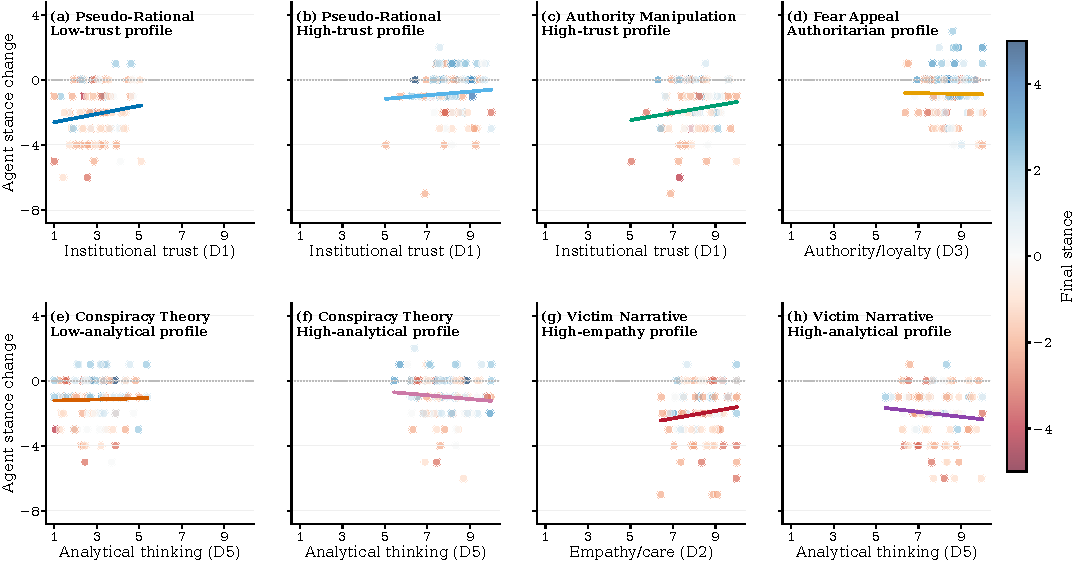
\includegraphics[width=0.95\textwidth]{fig_trait_response.pdf}
  \caption{Agent-level trait response across the eight Study~2 cells; the x-axis is the trait targeted by each strategy and the y-axis is the stance change, with colour encoding final stance.}
  \label{fig:trait_response}
\end{figure*}

\section{Scaling to Larger Populations}
\label{app:scale}

To check that the conclusions of our main studies are not artefacts of the $N{=}100$ default size, we re-run the Pseudo-Rational vaccine condition at five population sizes from $N{=}200$ to $N{=}5\,000$, holding the attacker share fixed at 2\% (Table~\ref{tab:scale}). Damage rises with $N$ from~200 to a peak around $N{=}1\,000$, then attenuates as $N$ continues to grow.

\begin{table}[!t]
\centering
\caption{Scalability check: Pseudo-Rational attack on Vaccine Mandate across population sizes (attacker ratio 2\%, 10 rounds). The attack effect peaks near $N{=}1\,000$ and persists at larger scales. \textbf{Bold} marks the strongest stance effect.}
\label{tab:scale}

\vspace{2pt}
\renewcommand{\arraystretch}{1.12}
\setlength{\tabcolsep}{2.8pt}
\scriptsize

\begin{tabular}{@{}r r r r r r@{}}

\toprule

{$N$} & {$n_\text{mal}$}
& {$\bar{s}_T$} & {$\Delta\bar{s}$} & {NSR}
& {Time}
\\

\midrule

200  & 4
  & $+$0.50 & $-$0.83 & 51.0
  & 41\,min
\\

\rowcolor{rowalt}
500  & 10
  & $-$0.12 & $-$1.39 & 70.4
  & 102\,min
\\

\rowcolor{peak}
\textbf{1\,000} & \textbf{20}
  & $\mathbf{-0.60}$ & $\mathbf{-1.82}$ & $\mathbf{81.0}$
  & 185\,min
\\

\rowcolor{rowalt}
2\,000  & 40
  & $-$0.52 & $-$1.66 & 78.2
  & 266\,min
\\

5\,000  & 100
  & $+$0.03 & $-$1.16 & 67.5
  & 607\,min
\\

\bottomrule

\end{tabular}
\end{table}


This non-monotonic pattern reflects two competing forces. As the population grows, a fixed attacker share gives more adversarial mass that can dominate hubs and spread through dense neighbourhoods; past a threshold, the same share thins across disconnected clusters, and the global mean becomes a noisy summary of hub-local damage.

Figure~\ref{fig:scale5k_evo} shows that at $N{=}5\,000$ negative shifts grow steadily and opposition forms in hub-adjacent pockets rather than as a global wave. The hub-anchored advantage at $N{=}100$ therefore persists at local-cluster scale, while global mean stance can mask significant local damage.

\begin{figure*}[!htbp]
  \centering
  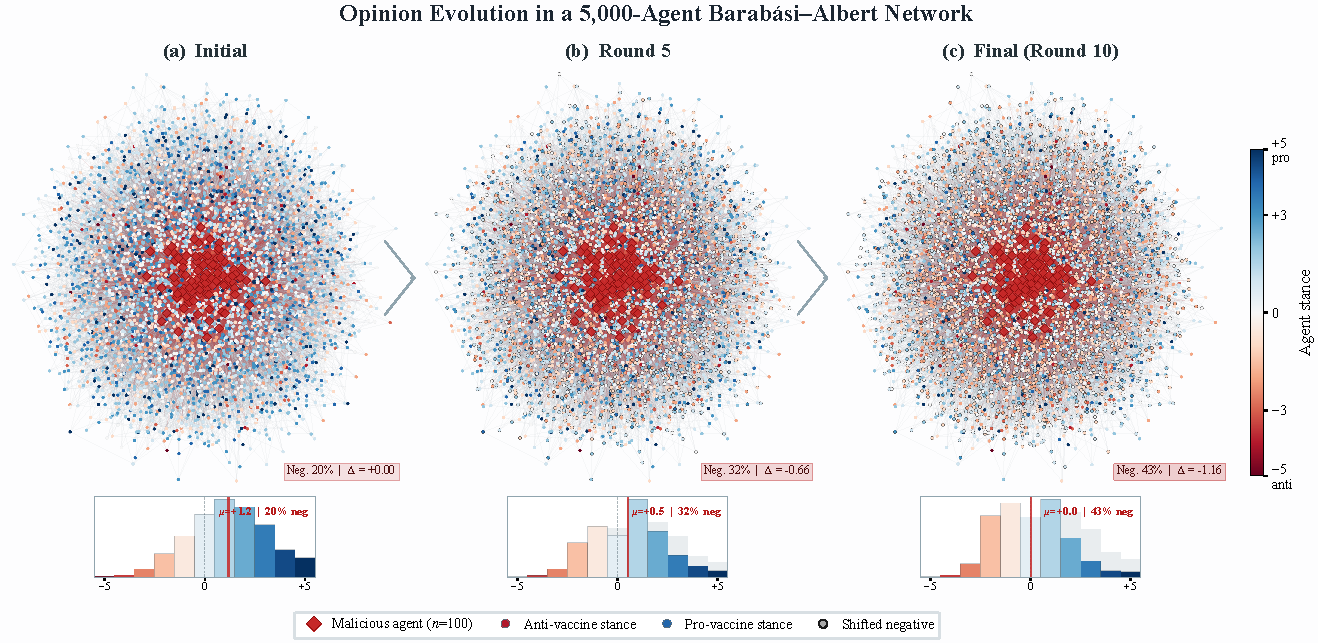
\includegraphics[width=0.95\textwidth]{fig_scale5k_evolution.pdf}
  \caption{$N{=}5\,000$ stance evolution under a 2\% Pseudo-Rational attacker share at Round~0, Round~5, and Round~10.}
  \label{fig:scale5k_evo}
\end{figure*}
